\documentclass[10pt]{article}

\usepackage{fullpage}
\usepackage{amsmath}
\usepackage{amssymb}
\usepackage{amsthm}
\usepackage{fancyhdr}
\usepackage{algorithm}
\usepackage{algorithmic}
\usepackage{bm}
\usepackage{framed}
\usepackage{graphicx}
\usepackage{multirow}
\usepackage{hyperref}
\usepackage{natbib}
\usepackage[usenames,dvipsnames]{xcolor}
% \usepackage[UTF8]{ctex}


\newtheorem{theorem}{Theorem}[section]
\newtheorem{lemma}[theorem]{Lemma}
\newtheorem{corollary}[theorem]{Corollary}
\newtheorem{proposition}[theorem]{Proposition}
\newtheorem{definition}[theorem]{Definition}
\newtheorem{conjecture}[theorem]{Conjecture}
\newtheorem{remark}[subsection]{Remark}

%%
\newcommand\numberthis{\addtocounter{equation}{1}\tag{\theequation}}

%% define new symbols
\def\bx{\bm{x}}
\def\bb{\bm{b}}
\def\ba{\bm{a}}
\def\bc{\bm{c}}
\def\bf{\bm{f}}
\def\by{\bm{y}}
\def\bu{\bm{u}}
\def\bv{\bm{v}}
\def\BW{\bm{W}}
\def\BA{\bm{A}}
\def\bz{\bm{z}}
\def\BZ{\bm{Z}}
\def\BH{\bm{H}}
\def\BL{\bm{L}}
\def\BU{\bm{U}}
\def\BV{\bm{V}}
\def\BB{\bm{B}}
\def\BC{\bm{C}}
\def\BD{\bm{D}}
\def\BE{\bm{E}}
\def\BW{\bm{W}}
\def\BQ{\bm{Q}}
\def\BG{\bm{G}}
\def\BA{\bm{A}}
\def\BX{\bm{X}}
\def\BY{\bm{Y}}
\def\BQ{\bm{Q}}
\def\BI{\bm{I}}
\def\BR{\bm{R}}

%% define new brackets
\def\la{\left\langle}
\def\ra{\right\rangle}
\def\ln{\left\|}
\def\rn{\right\|}
\def\lb{\left(}
\def\rb{\right)}
\def\lsb{\left[}
\def\rsb{\right]}
\def\lcb{\left\{}
\def\rcb{\right\}}

%%
\DeclareMathOperator*{\argmin}{arg\,min}
\DeclareMathOperator*{\argmax}{arg\,max}

%%
\title{Project-2 Report of ``Neural Network and Deep Learning''}
\author{Jialun Shen\\ 16307110030}
\date{}

\begin{document}
\maketitle
%------------------------------------
%\begin{abstract}
%\end{abstract}
%-------------------------------------
%=====================
\section{Train a Network on CIFAR-10}

\subsection{Introduction}

CIFAR-10~\citep{krizhevsky2009learning} is a widely used dataset for visual recognition task. 
% The CIFAR-10 dataset (Canadian Institute ForAdvanced Research) is a collection of images that are commonly used to train machine learning and computervision algorithms. 
% It is one of the most widely used datasets for machine learning research. 
% The CIFAR-10 dataset contains 60,000 32$\times$32 color images in 10 different classes. The 10 different classes represent airplanes, cars, birds, cats, deer, dogs, frogs, horses, ships, and trucks (as shown in Figure 1). There are 6,000 images of each class. 
% Since the images in CIFAR-10 are low-resolution (32 $\times$ 32), this dataset can allow us to quickly try our models to see whether it works.
In this project, I trained neural network models on CIFAR-10 to optimize performance. 
The default hyperparameter setting is shown in \autoref{tab:hyperparameter}.
In the following sections, I perform ablation experiments to test the effects of each hyperparameters.

\begin{table}[htb]
\centering
\caption{Default Hyperparameter Setting}
\begin{tabular}{c|c}
\hline
\textbf{Hyperparameter}   & \textbf{Value}      \\ \hline
epoch     & 50         \\
batch size   & 128         \\
initial learnig rate       & 0.1            \\
weight decay coefficient for L2 regularization      & 0.0005            \\
activation function        & ReLU        \\
optimizer  & SGD(with momentum)  \\
% scheduler & multisteplr \\
model & ResNet34 \\
ResNet 1st convolution layer kernel\_size, stride, padding & 7,2,3 \\
data augmentation  & no augmentation  \\
hidden layer size & no hidden layer \\ 
dropout probability & no dropout \\
\hline
\end{tabular}
\label{tab:hyperparameter}
\end{table}

\subsection{Network Structure}

The baseline model I use is ResNet~\citep{he2016deep}, which uses residual blocks and resiudual connections to avoid the problem of vanishing gradients. I first tried several public available versions of ResNet, which have different model depth or width. A deeper model usually takes more time to train. Also, I found that training accuracy is generally higher than validation accuracy, which shows the existence of over-fitting.

The final validation accuracy of each model is shown in \autoref{tab:result-model}. We can see that their performances are quite close (around 75\%) in this task, deeper models do not always show better performance. 

\begin{table}[htb]
\centering
\caption{Result: Different model depth/width}
\begin{tabular}{c|c|c}
\hline
\textbf{Model name}   & \textbf{Validation accuracy(\%)}    & \textbf{Time(sec)}  \\ \hline
ResNet18     & 75.22     & 451    \\
ResNet34 (default)   &  75.05   & 654     \\
ResNet50       & 76.50    & 991        \\
ResNet101      & 75.45    & 1505      \\
ResNet152        & 76.05   & 2033    \\
Wide ResNet-50-2~\citep{zagoruyko2016wide}  & 75.42 & 2327 \\
ResNeXt-50 32x4d~\citep{xie2017aggregated} & \textbf{77.46} &1189 \\
\hline
\end{tabular}
\label{tab:result-model}
\end{table}

Note that the original ResNet uses a $7\times 7$ convolution layer as the first layer, which is a fairly big kernal size for CIFAR-10, in which images have the size of $32\times 32$. Therefore, I modified the first convolution layer, including its kernal size, stride and padding. 
The modifications and results are shown in \autoref{tab:result-conv1}. We can see that a smaller kernal can represent the features from the image better than a bigger kernal. In the following experiments, I set the first convolution layer's kernel\_size, stride, padding to be (3, 1, 1), and use model ResNet34.

\begin{table}[htb]
\centering
\caption{Result: Different 1st convolution layer}
\begin{tabular}{c|c|c}
\hline
\textbf{kernel\_size, stride, padding}   & \textbf{Validation accuracy(\%)}   & \textbf{Time(sec)}   \\ \hline
7, 2, 3 (default)     & 75.05   & 654      \\
7, 2, 1   &  75.15     & 650   \\
7, 1, 1       & 77.59    & 766        \\
5, 2, 1      & 75.15    & 655       \\
5, 1, 1        & 78.41  & 903     \\
3, 1, 1  & \textbf{79.07} & 979 \\
\hline
\end{tabular}
\label{tab:result-conv1}
\end{table}

\subsection{Data Augmentation}

I tried two different kinds of data augmentation: (1) RandomGrayscale and (2) RandomCrop+HorizontalFlip. Their results compared to model without data augmentation is shown in \autoref{tab:result-data}. 
We can see that with RandomCrop+HorizontalFlip data augmentation, the model performance improves greatly.

\begin{table}[htb]
\centering
\caption{Result: Different data augmentation}
\begin{tabular}{c|c|c}
\hline
\textbf{Data augmentation type}   & \textbf{Validation accuracy(\%)}   & \textbf{Time(sec)}   \\ \hline
no augmentation (default)     & 79.07   & 979      \\
RandomGrayscale   &  79.91     & 979   \\
RandomCrop+HorizontalFlip      & \textbf{84.40}    & 980        \\
\hline
\end{tabular}
\label{tab:result-data}
\end{table}

\subsection{Optimizer}

I tried different optimizers, with the same initial learning rate of 0.1.
% and scheduler multisteplr. 
The result is shown in \autoref{tab:result-optim}. Several optimizers failed to converge, maybe due to sensitiveness to initial learning rate.

\begin{table}[htb]
\centering
\caption{Result: Different optimizers}
\begin{tabular}{c|c|c}
\hline
\textbf{Optimizer}   & \textbf{Validation accuracy(\%)}   & \textbf{Time(sec)}   \\ \hline
SGD(with momentum) (default)     & \textbf{79.07}   & 979      \\
Adagrad   &  77.17     & 970   \\
RMSprop      & 35.89    & 1011        \\
Adadelta     & 72.37    & 1050       \\
Adam        & 26.77  & 1017     \\
\hline
\end{tabular}
\label{tab:result-optim}
\end{table}

\subsection{Activation Function}

I tried different activation functions for all the layers. The result is shown in \autoref{tab:result-activation}, which are very close. So I choose to use the original activation funciton ReLU.

\begin{table}[htb]
\centering
\caption{Result: Different activation functions}
\begin{tabular}{c|c|c}
\hline
\textbf{activation function}   & \textbf{Validation accuracy(\%)}   & \textbf{Time(sec)}   \\ \hline
ReLU (default)     & 79.07   & 979      \\
ELU   &  79.06    & 979   \\
LeakyReLU     &   79.29  &  979       \\
RReLU    &  \textbf{79.50}   &   998     \\
Sigmoid        &  77.32 &  979    \\
Tanh       &  79.18 &   980   \\
\hline
\end{tabular}
\label{tab:result-activation}
\end{table}

\subsection{Add Extra Hidden Layer with Dropout and Batch Normalization}

I tried to add extra layers, including a hidden layer, a batch normalization layer and a dropout layer. I tested different hidden layer sizes, but did not see much improvement, as shown in \autoref{tab:result-hidden}. 
By further comparing the result with data augmentation with that in \autoref{tab:result-data}, the model performs even worse with extra layers.

\begin{table}[htb]
\centering
\caption{Result: Different hidden layer size}
\begin{tabular}{c|c|c}
\hline
\textbf{hidden layer size}   & \textbf{Validation accuracy(\%)}   & \textbf{Time(sec)}   \\ \hline
no hidden layer (default)     & 79.07   & 979      \\
10   &  79.60     & 980   \\
20      & 77.30    & 978        \\
50     & 79.54    & 980       \\
100        & 79.23  & 982     \\
10, with data augmentation method 2        & \textbf{81.01}  & 979     \\
10, with data augmentation method 2, ResNeXt-50 32x4d & 80.60 & 1873 \\
\hline
\end{tabular}
\label{tab:result-hidden}
\end{table}

\subsection{Learning Rate}

I tried different initial learning rates. In this section, I use ResNet34 with data augmentation method 2, optimizer is SGD(with momentum). Experiments show that learning rate is an important hyperparameter that has a great influence on the model perfromance, as shown in \autoref{tab:result-lr}. The optimal learning rate is 0.01. In addition, Adam optimizer still performs worse than SGD(with momentum).

\begin{table}[htb]
\centering
\caption{Result: Different learning rate}
\begin{tabular}{c|c|c}
\hline
\textbf{Learning rate}   & \textbf{Validation accuracy(\%)}   & \textbf{Time(sec)}   \\ \hline
0.1 (default)     & 84.40   & 980      \\
0.05   &  86.01     & 977   \\
0.01      & \textbf{87.09}    & 978        \\
0.005     & 85.81    & 978       \\
0.001        & 76.71  & 978     \\
0.01, with optimizer Adam       & 68.95  & 1001     \\
0.005, with optimizer Adam       & 76.63  & 1006     \\
\hline
\end{tabular}
\label{tab:result-lr}
\end{table}

\subsection{Batch Size}

I tried different batch sizes, as shown in \autoref{tab:result-batch}. Smaller batch size usualliy requires longer training time. I choose batch size to be 64 for the following experiments.

\begin{table}[htb]
\centering
\caption{Result: Different batch size}
\begin{tabular}{c|c|c}
\hline
\textbf{Batch size}   & \textbf{Validation accuracy(\%)}   & \textbf{Time(sec)}   \\ \hline
256 & 85.85 & 932 \\
128  (default)    & 87.09    & 978        \\
64 & \textbf{87.97} & 1210 \\
32 & 87.15 & 1920 \\
\hline
\end{tabular}
\label{tab:result-batch}
\end{table}

\subsection{Number of Epoch}

Epoch is the number of times the model will see all the training data during training.
With other hyperparameters fixed, training time is propotional to the number of epoch. The experiment result is shown in \autoref{tab:result-epoch}. Model performance goes up as epoch increases, but the improvement gradually slows down.

\begin{table}[htb]
\centering
\caption{Result: Different number of epoch}
\begin{tabular}{c|c|c}
\hline
\textbf{Epoch}   & \textbf{Validation accuracy(\%)}   & \textbf{Time(sec)}   \\ \hline
10 & 80.90 & 242 \\
50  (default)    & 87.97    & 1210        \\
100 & \textbf{89.08} & 2417 \\
\hline
\end{tabular}
\label{tab:result-epoch}
\end{table}


\subsection{Final Model}

The final model I choose is ResNet34, with optimizer SGD(with momentum)
with the first convolution layer's kernel\_size, stride, padding being (3, 1, 1),
and RandomCrop+HorizontalFlip data augmentation, trained with 100 epochs. (Detailed hyperparameter setting shown in \autoref{tab:hyperparameter-final}.) Its validation accuracy is 89.08\%, which has the best performance among all the models tested above. I plotted training accuracy/loss and validation accuracy/loss during training as \autoref{fig:cifar}.

\begin{table}[htb]
\centering
\caption{Final Model Hyperparameter Setting}
\begin{tabular}{c|c}
\hline
\textbf{Hyperparameter}   & \textbf{Value}      \\ \hline
epoch     & 100         \\
batch size   & 64         \\
initial learnig rate       & 0.01            \\
weight decay coefficient for L2 regularization      & 0.0005            \\
activation function        & ReLU        \\
optimizer  & SGD(with momentum)  \\
% scheduler & multisteplr \\
model & ResNet34 \\
ResNet 1st convolution layer kernel\_size, stride, padding & 3,1,1 \\
data augmentation  & RandomCrop+HorizontalFlip  \\
hidden layer size & no hidden layer \\ 
dropout probability & no dropout \\
\hline
\end{tabular}
\label{tab:hyperparameter-final}
\end{table}

\begin{figure}[htb]
  \centering
  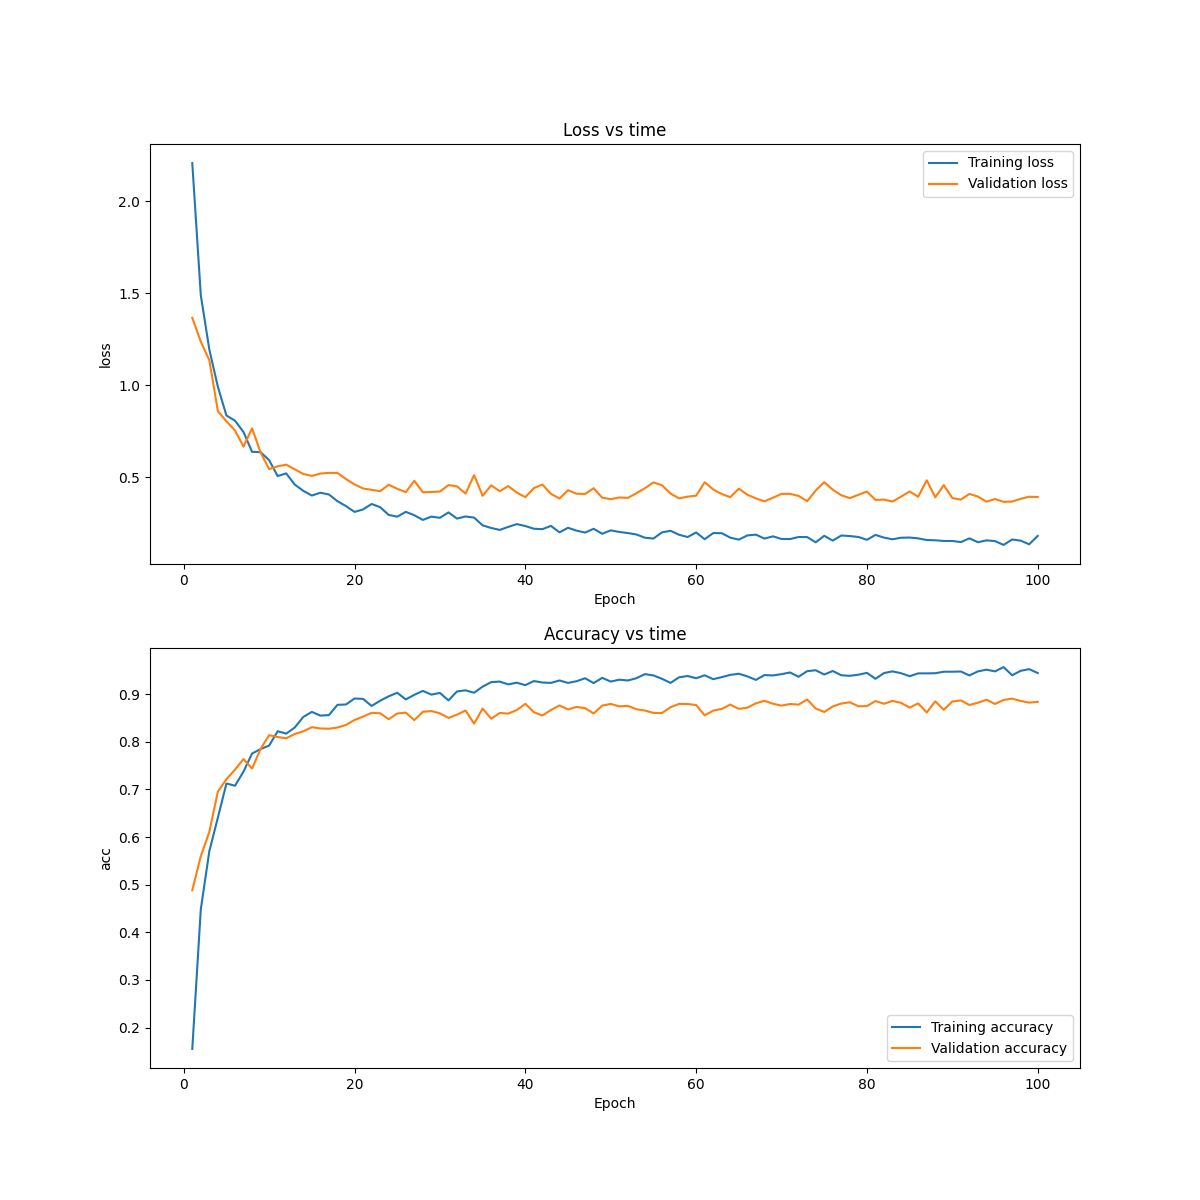
\includegraphics[width=0.9\textwidth]{figures/resnet34_aug2_lr1e-2_conv1311_batch64_epoch100.png}
  \caption{%
    Loss and accuracy vs time}
  \label{fig:cifar}
\end{figure}

\section{VGG-A with and without Batch Normalization}

\subsection{Training Result}

Original VGG-A has 9,750,922 parameters, and VGG-A with batch normalization has 9,758,474 parameters.

The networks are trained for 20 epochs with different learning rates. The maximum validation accuracy of each model is shown in \autoref{tab:result-vgg}. In most cases, VGG-A with batch normalization performs better than VGG-A without it.


\begin{table}[htb]
\centering
\caption{Result: VGG-A with and withoput BN}
\begin{tabular}{c|c|c}
\hline
\textbf{LR}   & \textbf{Val acc without BN(\%)}   & \textbf{Val acc with BN(\%)}   \\ \hline
0.001   & 77.27 & 82.05 \\
0.002   & 73.80 & 82.22 \\
0.0001  & 76.62 & 73.27 \\
0.0005  & 78.73 & 81.47 \\
\hline
\end{tabular}
\label{tab:result-vgg}
\end{table}

\subsection{Loss Landscape}

Loss landscape of models trained above is shown in \autoref{fig:loss-landscape}. We can see that VGG-A with BN converges faster, and has a smaller fluctuation with different learning rates.

\begin{figure}[htb]
  \centering
  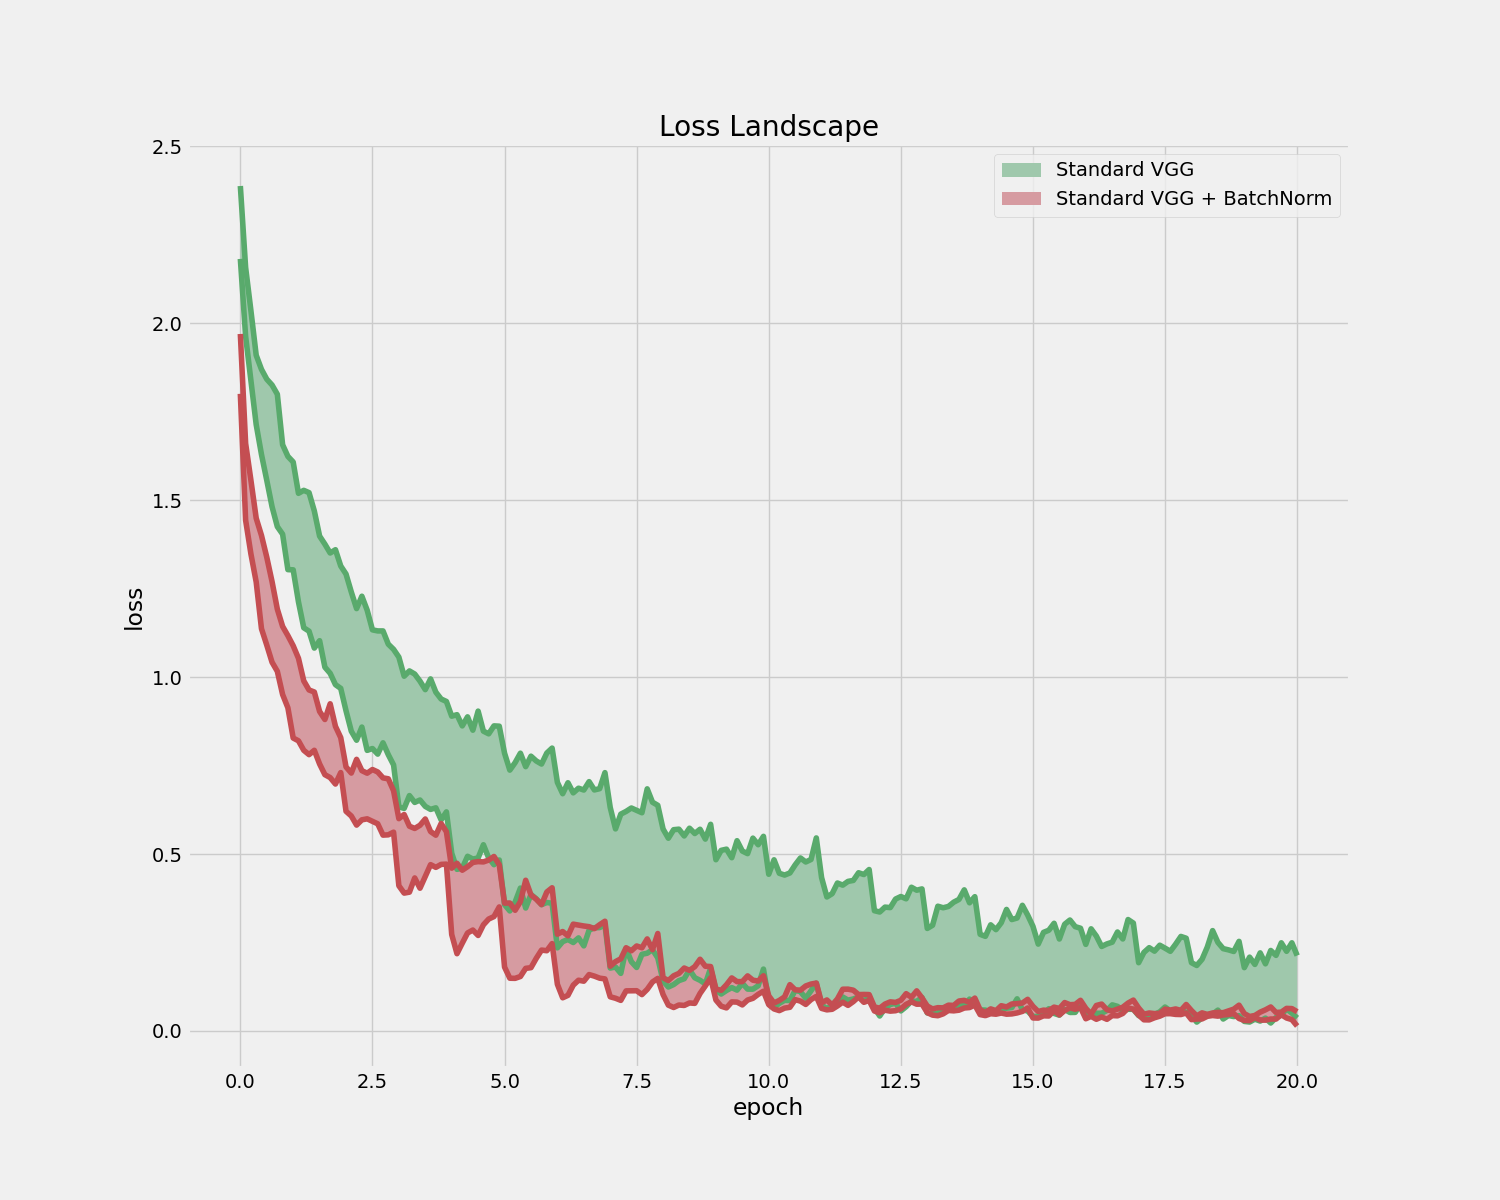
\includegraphics[width=0.9\textwidth]{figures/loss_landscape.png}
  \caption{%
    Loss Landscape}
  \label{fig:loss-landscape}
\end{figure}

\subsection{Gradient Predictiveness}

Gradient predictiveness of models trained above is shown in \autoref{fig:grad-predictiveness}. With BN, gradient predictiveness of VGG-A becomes much more stable than that without BN.

\begin{figure}[htb]
  \centering
  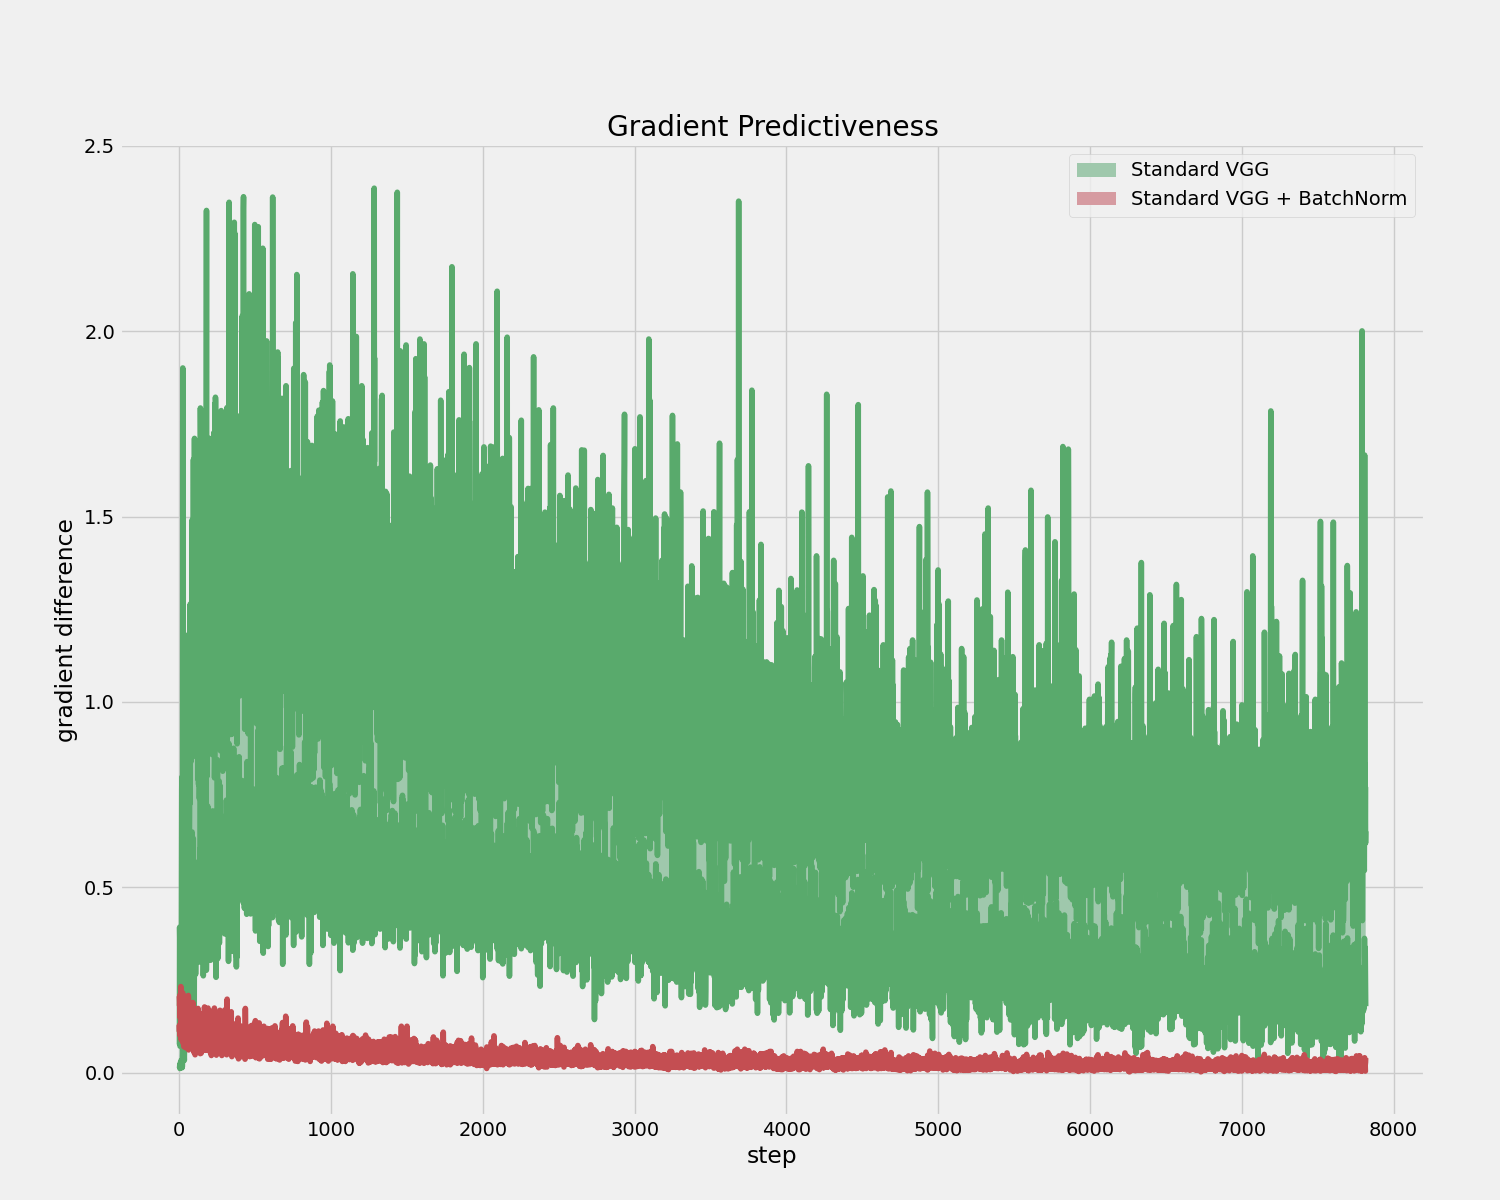
\includegraphics[width=0.9\textwidth]{figures/grad_predictiveness.png}
  \caption{%
    Gradient Predictiveness}
  \label{fig:grad-predictiveness}
\end{figure}

\subsection{``Effective'' $\beta$-Smoothness}
``Effective'' $\beta$-Smoothness of models trained above is shown in \autoref{fig:beta-smoothness}. We can see that, with BN, ``effective'' $\beta$-smoothness of VGG-A is also much more stable than that without BN.


\begin{figure}[htb]
  \centering
  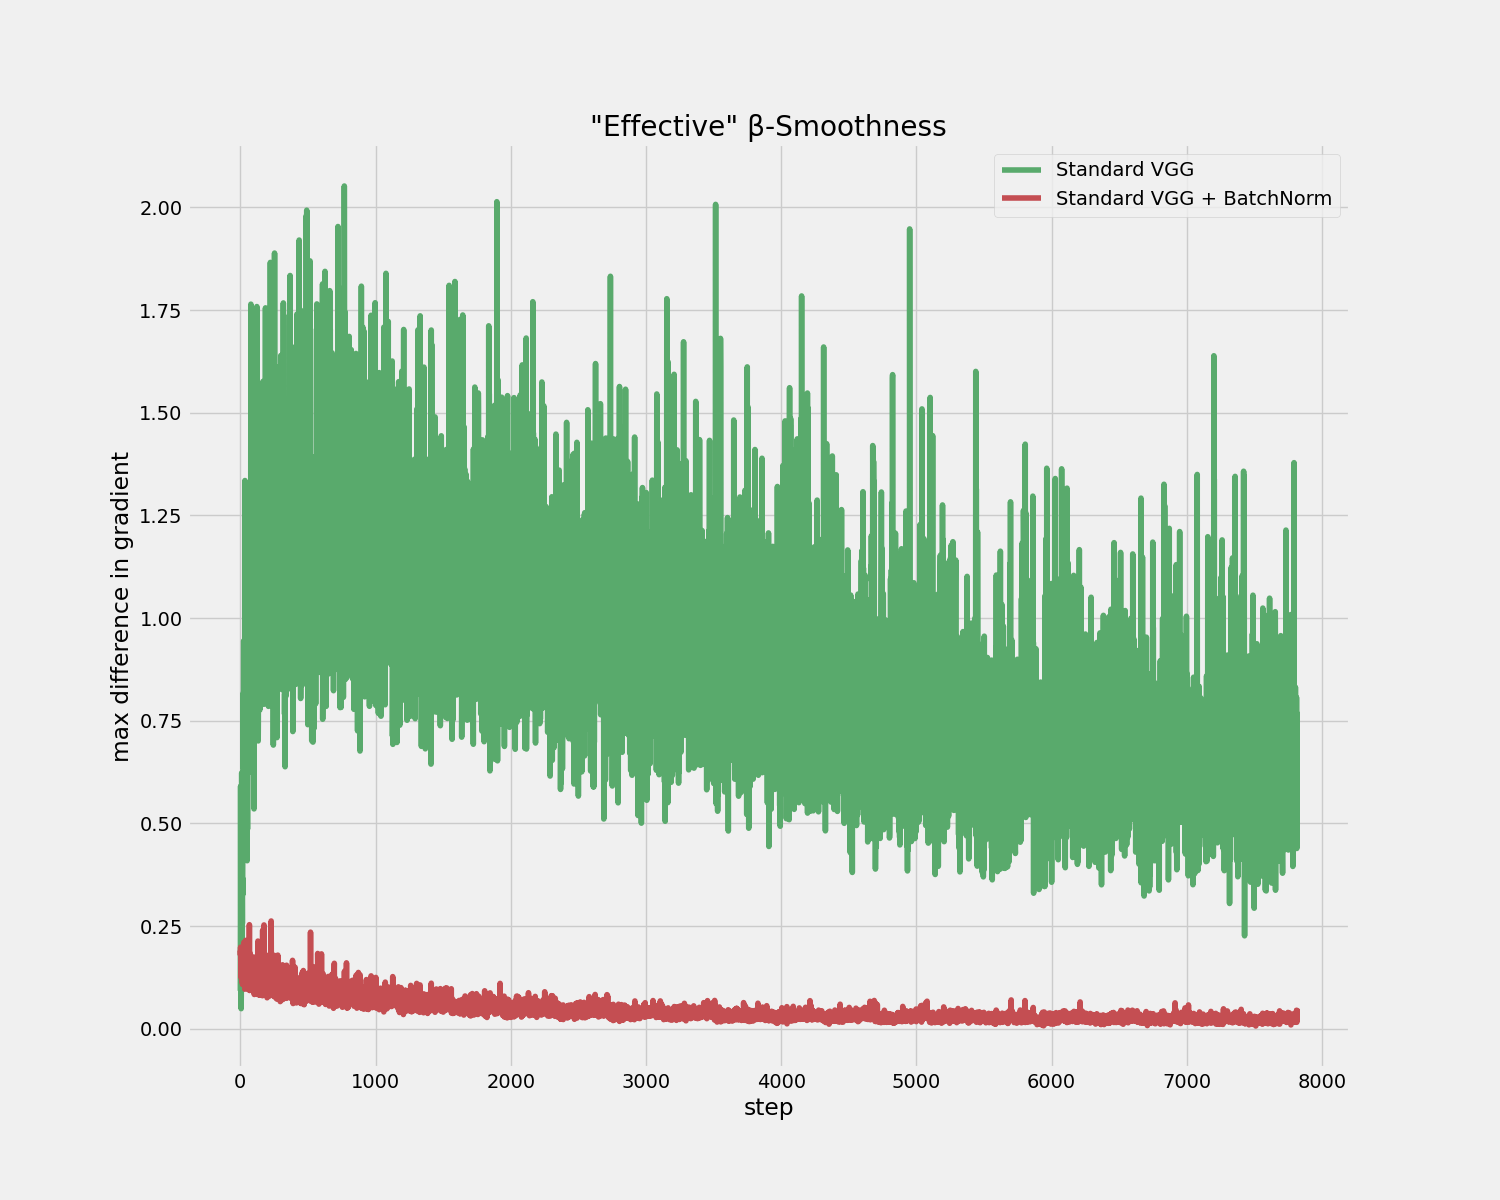
\includegraphics[width=0.9\textwidth]{figures/beta_smoothness.png}
  \caption{%
    ``Effective'' $\beta$-Smoothness}
  \label{fig:beta-smoothness}
\end{figure}


%-------------------------------------
%=====================
\newpage
\bibliographystyle{plain}
\interlinepenalty=10000
\bibliography{reference}

\end{document}
